\documentclass[preview]{standalone}
\usepackage{amsmath}
\usepackage{amssymb}
\usepackage{stellar}
\usepackage{definitions}
\usepackage{bettelini}
\usepackage{tikz}
\begin{document}
\id{diffeq-undetermined-coefficients}
\genpage
\section{Undetermined coefficients}

\begin{snippettheorem}{diffeq-undetermined-coefficients-theorem}{Exponential-polynomial forcing}
    Let \(P\in\realnumbers[\lambda]\) be monic of degree \(k\geq1\),
    let \(\mu\in\complexnumbers\), and let \(Q\neq0\) be a polynomial of degree \(m\).
    Write \(r\) for the multiplicity of \(\mu\) as a root of \(P\),
    with \(r=0\) when \(P(\mu)\neq0\).
    The equation
    \[
        P(D)y=e^{\mu x}Q(x)
    \]
    has a particular solution \(y_*=x^re^{\mu x}R(x)\),
    where \(R\) is a polynomial of degree \(m\).
    Its coefficients are uniquely determined within this ansatz.
\end{snippettheorem}

\begin{snippetproof}{diffeq-undetermined-coefficients-proof}{diffeq-undetermined-coefficients-theorem}{Exponential-polynomial forcing}
    The shift identity is
    \[
        P(D)(e^{\mu x}v)=e^{\mu x}P(D+\mu)v.
    \]
    Write \(P(\mu+\lambda)=\lambda^rS(\lambda)\), where \(S(0)\neq0\).
    The map \(D^r\) takes \(x^rR(x)\), \(\deg R\leq m\), bijectively onto
    all polynomials of degree at most \(m\). On that space \(S(D)\) is invertible,
    since it is triangular with nonzero diagonal \(S(0)\).
    Hence \(S(D)D^r(x^rR)=Q\) uniquely determines \(R\).
    The nonzero leading coefficient of \(Q\) forces \(\deg R=m\).
\end{snippetproof}

\begin{snippetcorollary}{diffeq-polynomial-forcing}{Polynomial forcing}
    Let \(P\) be the characteristic polynomial of a constant-coefficient
    equation \(P(D)y=Q_m(x)\), where \(Q_m\) is a nonzero polynomial of degree \(m\).
    If zero is not a root of \(P\), a particular solution is a polynomial of degree \(m\).
    If zero has multiplicity \(r\), a particular solution is \(x^rR_m(x)\)
    with \(R_m\) of degree \(m\).
\end{snippetcorollary}

\begin{snippetcorollary}{diffeq-exponential-forcing}{Exponential forcing}
    For a constant-coefficient equation \(P(D)y=e^{\mu x}\),
    if \(P(\mu)\neq0\), a particular solution is \(e^{\mu x}/P(\mu)\).
    If \(\mu\) is a root of multiplicity \(r\geq1\), a particular solution is
    \[
        y_*=\frac{x^re^{\mu x}}{P^{(r)}(\mu)}.
    \]
\end{snippetcorollary}

\begin{snippetcorollary}{diffeq-oscillating-forcing}{Oscillating forcing}
    Let \(P\) have real constant coefficients and let
    \(\alpha,A,B\in\realnumbers\), \(\beta>0\).
    For
    \[
        P(D)y=e^{\alpha x}\bigl(A\sin(\beta x)+B\cos(\beta x)\bigr),
    \]
    let \(r\) be the multiplicity of \(\alpha+i\beta\) as a root of \(P\),
    or zero if it is not a root. A particular solution can be found in the form
    \[
        y_*=x^re^{\alpha x}\bigl(C\sin(\beta x)+D\cos(\beta x)\bigr).
    \]
\end{snippetcorollary}

\begin{snippetproposition}{diffeq-forcing-superposition}{Adding forcing terms}
    For a fixed linear differential operator \(L\), if \(L[y_j]=b_j\)
    on an interval for \(1\leq j\leq m\), then
    \(L[\sum_j y_j]=\sum_j b_j\).
    Thus for forcing \(x^2+\cos x-e^{3x}\), one may find a particular
    solution for each of the three terms and add them.
\end{snippetproposition}

\section{Resonance}

\begin{snippetexample}{diffeq-forced-oscillator-example}{An undamped forced oscillator}
    Consider \(y''+\omega^2y=\sin(\ell x)\), with \(\omega,\ell>0\).
    The homogeneous solution is \(y_h=c_1\cos(\omega x)+c_2\sin(\omega x)\).

    If \(\ell\neq\omega\), try \(y_*=C\cos(\ell x)+D\sin(\ell x)\).
    Since \(y_*''=-\ell^2y_*\),
    \[
        y_*''+\omega^2y_*=(\omega^2-\ell^2)y_*.
    \]
    Coefficient comparison gives \(C=0\), \(D=1/(\omega^2-\ell^2)\), hence
    \[
        y=c_1\cos(\omega x)+c_2\sin(\omega x)
          +\frac{\sin(\ell x)}{\omega^2-\ell^2}.
    \]

    If \(\ell=\omega\), resonance requires the factor \(x\):
    \[
        y_*=x\bigl(C\cos(\omega x)+D\sin(\omega x)\bigr).
    \]
    Direct differentiation gives
    \[
        y_*''+\omega^2y_*
        =2D\omega\cos(\omega x)-2C\omega\sin(\omega x).
    \]
    Thus \(D=0\), \(C=-1/(2\omega)\), and
    \[
        y=c_1\cos(\omega x)+c_2\sin(\omega x)
          -\frac{x}{2\omega}\cos(\omega x).
    \]
    The original schematic drawing illustrates a linearly growing oscillation
    envelope, not the precise phase or frequency of this particular solution.
\begin{center}
        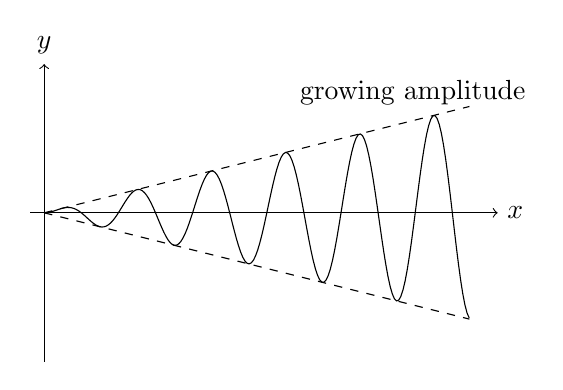
\begin{tikzpicture}[scale=0.9]
            \draw[->] (-0.2,0) -- (6.4,0) node[right] {\(x\)};
            \draw[->] (0,-2.1) -- (0,2.1) node[above] {\(y\)};
            \draw[domain=0:6,samples=200] plot (\x,{0.25*\x*sin(6*\x r)});
            \draw[dashed] (0,0) -- (6,1.5);
            \draw[dashed] (0,0) -- (6,-1.5);
            \node at (5.2,1.7) {growing amplitude};
        \end{tikzpicture}
    \end{center}
\end{snippetexample}

\section{Complex forcing}

\begin{snippetexample}{diffeq-complex-forcing-example}{Taking real and imaginary parts}
    Let \(a_1,a_2,\alpha,\beta\in\realnumbers\) and consider
    \[
        y''+a_1y'+a_2y=e^{\alpha x}\sin(\beta x).
    \]
    Set \(\mu=\alpha+i\beta\), \(P(\lambda)=\lambda^2+a_1\lambda+a_2\).
    First solve the complex equation with right-hand side \(e^{\mu x}\).
    If \(P(\mu)\neq0\), try \(y_{*,c}=Ae^{\mu x}\).
    Then \(y_{*,c}'=A\mu e^{\mu x}\), \(y_{*,c}''=A\mu^2e^{\mu x}\), so
    \[
        A(\mu^2+a_1\mu+a_2)e^{\mu x}=e^{\mu x},\qquad
        A=\frac1{(\alpha+i\beta)^2+a_1(\alpha+i\beta)+a_2}.
    \]
    Because the coefficients are real, the desired particular solution is
    \(\operatorname{Im}(y_{*,c})\). For cosine forcing, take
    \(\operatorname{Re}(y_{*,c})\) instead.
    At a root \(\mu\) of multiplicity \(r\), use
    \(y_{*,c}=x^re^{\mu x}/P^{(r)}(\mu)\) before taking the appropriate part.
\end{snippetexample}

\end{document}
